\documentclass{article}
\usepackage[utf8]{inputenc}
\usepackage[export]{adjustbox}
\usepackage{subfig}
\usepackage{graphicx}
\usepackage{wrapfig}
\graphicspath {
	{images/}
}


\begin{document}
\title{System Service Design}
\author{Cardspark - Group 26}
\date{\today}
\maketitle  

Whereas before our users may have had to carry a lots of notes, we have to a mobile iOS to save them this effort and can be used in any spare moment.

\begin{center}
	\vspace{1mm}
	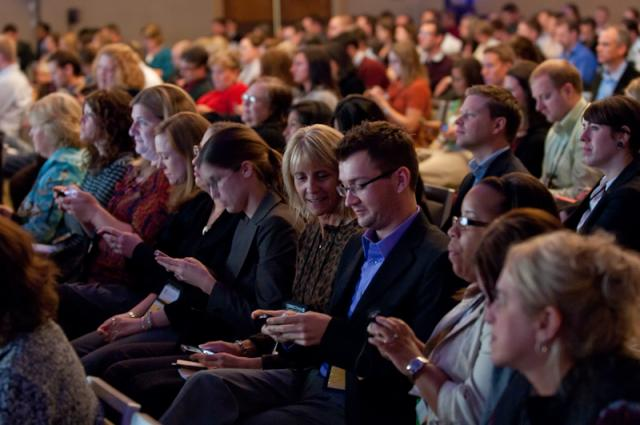
\includegraphics[scale=0.35]{public.jpg}
	\vspace{1mm}
\end{center}

Before users would have to transfer physical notes to each other, meaning only one person could have the notes at one time.  With Cardspark, they can collaborate in real time on the cards and always have access to them as they only need to know their emails.

\begin{center}
	\vspace{1mm}
	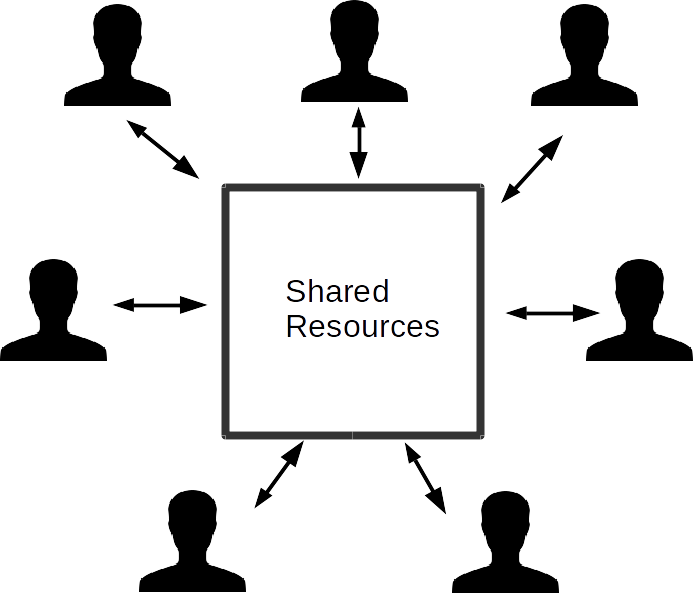
\includegraphics[scale=0.35]{shared.png}
	\vspace{1mm}
\end{center}

The use of Cardspark by our users means they can integrate photos they take and images they find into their notes whereas before these would need to be printed off or drawn.


\begin{center}
	\vspace{1mm}
	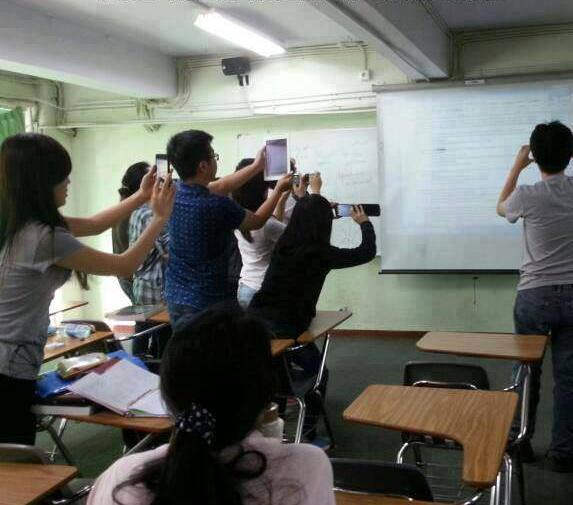
\includegraphics[scale=0.5]{camera.jpg}
	\vspace{1mm}
\end{center}

To stop people getting distracted when trying to learn/revise using our app, we added a built-in messenger feature along with a timer to help prevent outside sources on their phone or otherwise distracting them.

\begin{figure}[!ht]
  \centering
  \subfloat{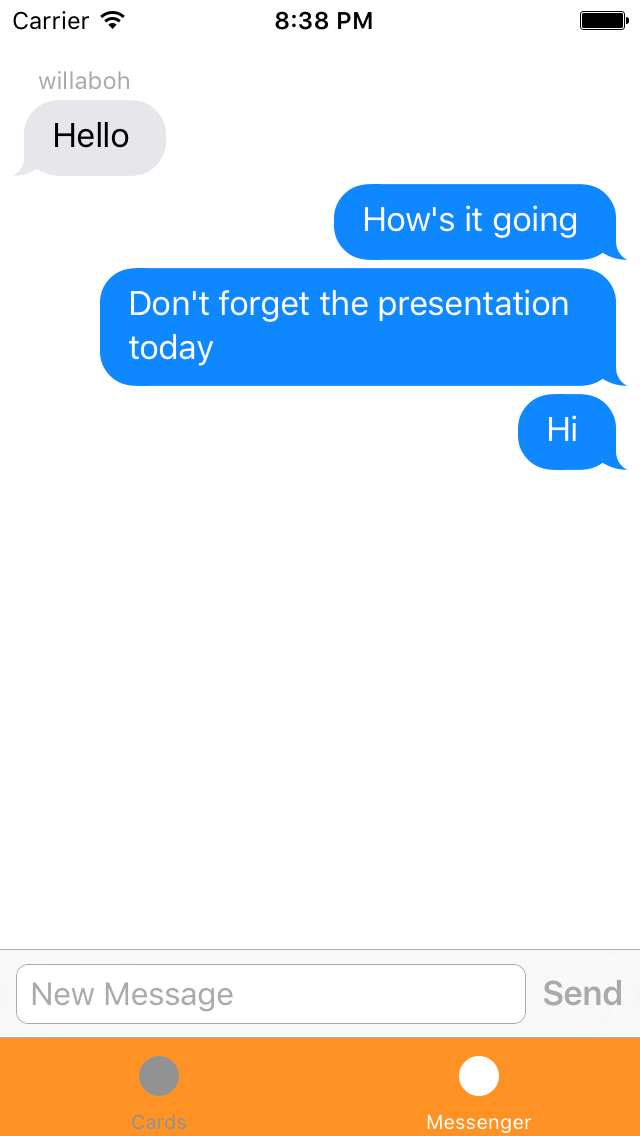
\includegraphics[scale=0.2]{mess.png}\label{fig:f1}}
  \hfill
  \subfloat{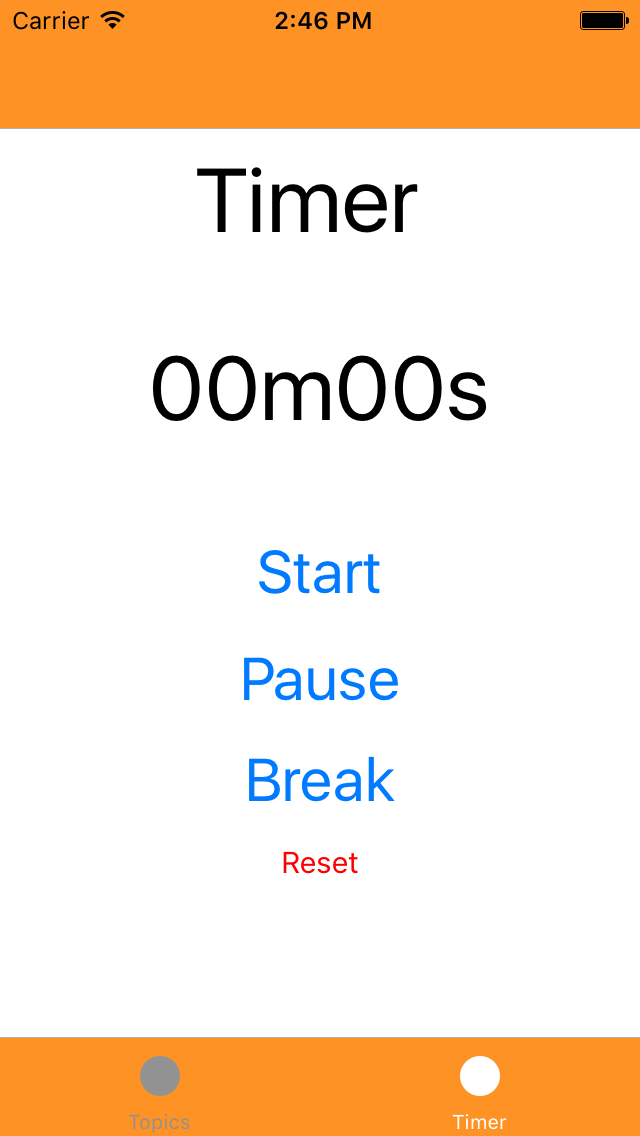
\includegraphics[scale=0.2]{timer.png}\label{fig:f2}}
\end{figure}


\end{document}
